\documentclass[border=5pt]{standalone}
\usepackage{tikz}
\begin{document}
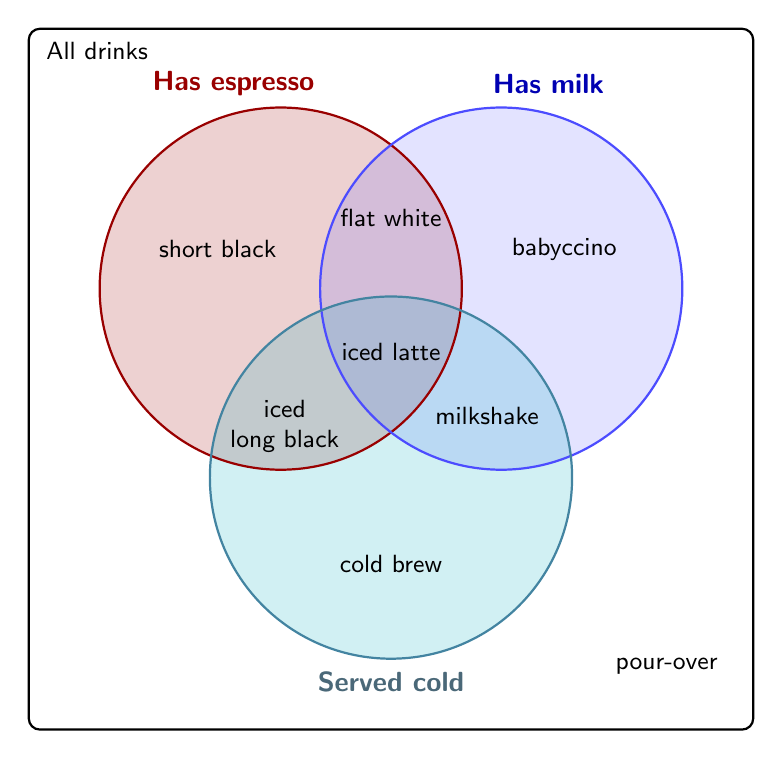
\begin{tikzpicture}[font=\sffamily\small]
  \def\r{2.3}
  \coordinate (A) at (0,0);      % espresso
  \coordinate (B) at (2.8,0);    % milk
  \coordinate (C) at (1.4,-2.4); % cold
  \draw[rounded corners, thick] (-3.2,-5.6) rectangle (6.0,3.3);
  \node[anchor=north west] at (-3.1,3.25) {All drinks};
  \fill[red!60!black, opacity=.18] (A) circle (\r);
  \fill[blue!60, opacity=.18] (B) circle (\r);
  \fill[cyan!70!green, opacity=.18] (C) circle (\r);
  \draw[thick, red!60!black] (A) circle (\r);
  \draw[thick, blue!70] (B) circle (\r);
  \draw[thick, cyan!60!black] (C) circle (\r);
  % circle labels
  \node[font=\sffamily\bfseries, red!60!black] at (-0.6,2.6) {Has espresso};
  \node[font=\sffamily\bfseries, blue!70!black] at (3.4,2.6) {Has milk};
  \node[font=\sffamily\bfseries, cyan!40!black] at (1.4,-5.0) {Served cold};
  % drinks
  \node at (-0.8,0.5) {short black};
  \node at (3.6,0.5) {babyccino};
  \node at (1.4,-3.5) {cold brew};
  \node at (1.4,0.9) {flat white};
  \node at (1.4,-0.8) {iced latte};
  \node[align=center] at (0.05,-1.75) {iced\\long black};
  \node at (2.62,-1.62) {milkshake};
  \node at (4.9,-4.8) {pour-over};
\end{tikzpicture}
\end{document}
